\documentclass[11pt]{article}

\usepackage{graphicx}
\usepackage{amsmath,amssymb}
\usepackage{graphbox}

\newcommand\numberthis{\addtocounter{equation}{1}\tag{\theequation}}

\usepackage{caption}
\usepackage{subcaption}
\usepackage{parskip}

\usepackage{physics}
\usepackage{slashed}

\usepackage[compat=1.1.0]{tikz-feynman}

\usepackage{pgffor}

\usepackage[margin=1in,footskip=0.25in]{geometry}

% Margins
\evensidemargin=0in
\oddsidemargin=0in
\textwidth=6.5in

%\setlength{\jot}{10pt}

\newcommand{\qe}[1]{
	\begin{center}
		\fbox{\parbox{0.9\textwidth}{#1}}
	\end{center}
}

\setlength{\jot}{8pt}


\title{Study of Relativistic Effects in Orbital Mechanics Using Numerical Methods}
\author{Axel Tibbling}
\date{ }


\begin{document}
\maketitle

%  Include nice image here

\section{Introduction}\label{sec:introduction}

\subsection{Theoretical background}

In general relativity (GR) is one of the more central and useful properties the \textit{metric}. We recall that in GR are there three spatial coordinates ($x, y, z$) and one time componen ($y$). These four quantities make ut a space time coordinate, which describes a spatial point in time. The universe can be thought of consisting of a grid-like blanket (mathematically it is called a \textit{manifold}) which describes the space time. The "blanket" can be be folded and creased describing disturbances made by massive objects in space. However, because the universe is infinite, where is origo found?

In the euclidian coordinate system vectors are used to describe the distance in a certain direction. In GR it is more useful to define a \textit{tangent basis}, which instead describes the change of the coordinates in a certain direction (simply put). To then describe distance, one cannot just study the vectors. This is where the metric comes in, as it describes how the manifold changes in certain directions. The notion of lengths the comes in the form of an infitesimal distance with the line segment \cite{guidry_2019}:

\begin{equation}
	ds^2 = g_{ij} du^i du^j
\end{equation}

where $g_{ij}$ are the components of the metric, and $du^i$ is the basis vectors. In GR is length (or \textit{proper length}) and so called \textit{proper time} isomorphic. Proper time describes the time of a clock following the line of interest on a manifold. The lines objects follow are called \textit{geodesics}, and are the lines which minimize the action which often are constructed by the metric. More explicitly, one creates the Lagrangian, and then by the least action principle, the Euler-Lagrange equations yield the equations of motion (EOM) that describe the geodesics \cite{guidry_2019}. 

% Do I want to have this here, or in the problem description?
In this paper we will study the Schwarzschild metric, which is used to describe the gravitational curvature around a black hole (or rather a massive object). It is expressed in polar coordinates around the massive point, and can be used to study how light rays and (smaller) massive objects travel along lines around more massive objects. Given in \cite{gould_2007, guidry_2019}, the Schwarzschild metric is

\begin{equation}\label{eq:schwarzschild-metric}
	d\sigma^2 = -d\tau^2 = - \left( 1 - \frac{2M}{r}\right)dt^2 + \left(1 - \frac{2M}{r}\right)^{-1} dr^2 + r^2 d\phi^2
\end{equation}

where $d\sigma$ is the proper distance and $d\tau$ is the proper time, while $M$ is the mass of the source of the gravitational curvature. Directly, there are two things that can be observed. Firstly, there is no angular dependence: it is has circular symmetry. Further, there is one singularity at $r_s = 2M$, which is commonly called the Schwarzschild radius \cite{guidry_2019}. 

In order to be able to numerically study this, the EOM is needed, which are given on page 760 in \cite{gould_2007}

\begin{align}\label{eq:eoms}
      		\frac{dr}{dt} &= \dot{r} \\
	\frac{d\dot{r}}{dt} &= \frac{4 M^3-4 M^2 r-4 M^2 r^3 \dot{\phi}^2+4 M r^4 \dot{\phi}^2-r^5 \dot{\phi}^2+r^2\left(M-3 M \dot{r}^2\right)}{(2 M-r) r^3} \\
	\frac{d\phi}{dt} &= \dot{\phi} \\
	\frac{d\dot{\phi}}{dt} &= \frac{2(-3M + r)\dot{r}\dot{\phi}}{(2M - r)r} \\
	\frac{dt}{dt} &= 1
\end{align}

and can be obtained using the Euler-Lagrange equations on \eqref{eq:schwarzschild-metric}. 

\subsection{The problem}
Numerical methods are a tool to model reality. In reality is Mercury close enough to the Sun for relativistic effects to affect tye system \cite{wiki_precession}. Thus will we calculate the orbit time and periohelion precession of Mercury around the Sun, and compare it to observed values.  

In order to solve the equations of motion we will use three different numerical integrators: Euler method, Backward Euler and Runge-Kutta 4 (RK4). In addition to the main goals, we also want to study how the integrators compare and will be done through analysis of energy conservation and error propagation.

In section \ref{sec:method} will the different numerical methods used be described and how the discritezation is done. Followed by that, in \ref{sec:results} will the orbit of Mercury be simulated, with the analysis of the integrators used.  Finally, in \ref{sec:disscussion} will the results be discussed, comparing the results and making concluding remarks. 



\section{Method}\label{sec:method}

\subsection{Integrators}

Before describing the integrators, we introduce the following notation for the state vector

\begin{equation}
	(x_1, x_2, x_3, x_4) := (r, \dot{r}, \phi, \dot{\phi})
\end{equation}

and is denoted by $\textbf{x}^n$, where $i$ denotes the current step. Furthermore, the function $\textbf{f}(\textbf{x})$ is then defined as the EOMs \eqref{eq:eoms}. Finally, the timestep is defined as $h$.  

\subsubsection{Euler method}
Being one of the simplest numerical integrators, it serves as a good foundation to compare the other methods to. As we will se does it behave better in some regards, but is generally found to be the lower limit of performance between the integrators. The equation defining this method is

\begin{equation}\label{eq:euler-method-equation}
	\textbf{x}^{n+1} = \textbf{x}^n + h \textbf{f}(\textbf{x}^n) 
\end{equation}


\subsubsection{Backward Euler method}

Because this method depends on the equations of motion and the derivative (Jacobian) of the as well, it was much more difficult to implement, and in the case that the EOM are slightly changed, one must recalculate the derivative, and hence reformulate the algorithm for Euler backward as well. This makes this method slightly inconvinient to use, but in the case, such as here, where only one system of equations are investigated, it is adequate practically. 

Just as in 1 dimesnion, Backward Euler here depends on Newton's method to solve for the next step. Here we have 4 dimensions, and the equation to be solved is 

\begin{equation}
	\mathbf{F}(\mathbf{x}^{n+1}) = \mathbf{x}^{{n+1}} - h \mathbf{f}(\mathbf{x}^{{n+1}}) - \mathbf{x}^n = 0
\end{equation}

To solve this equation, Newton's method must be employed. In order to use this method, the vector correspondant to the derivative must be used: the Jacobian. The algorithm is as follows: 

\begin{enumerate}
	\item Initialize $\textbf{x}^{n+1}_0$ with a good guess: pick $\textbf{x}^n$
	\item Calculate $\textbf{F} = \textbf{x}^{n+1}_{j} - \textbf{x}^{n} - h \textbf{f}(\textbf{x}^{n+1}_{j})$
	\item Calcuate the Jacobian $\mathcal{J}$ at the point $\textbf{x}^{n+1}_{j}$
	\item $\textbf{x}^{n+1}_{j+1} = \textbf{x}^{n+1}_{j} - \mathcal{J}^{-1} \textbf{F}$
	\item If $|\textbf{x}^{n+1}_{j+1} - \textbf{x}^{n+1}_{j}| \le $ threshold: next step is found.
	\item Else: return to step 2.
\end{enumerate}

where $j$ here is the step of the Newton's method. Note here that $t$ only depends on itself, and will thus not be handled in the numerical methods, as it is trivial.  

\subsubsection{Runge-Kutte 4 (RK4)}

Runge Kutta 4 is sort of an extension of the Euler Method, rather than calculating the timestep in one interval, RK4 does it in 4 steps. The method has the following equation:


\begin{align}
	\textbf{x}^{n+1} &= \frac{1}{6}h(k_1 + 2k_2 + 2k_3 + k_4) \textbf{x}^n \\
	k_1 &= \textbf{f}(\textbf{x}^n) \\
	k_2 &= \textbf{f}(\textbf{x}^n + \frac{1}{2}h k_1) \\
	k_3 &= \textbf{f}(\textbf{x}^n + \frac{1}{2}h k_2) \\
	k_4 &= \textbf{f}(\textbf{x}^n + h k_3)
\end{align}

The structure of the Euler method can be seen, but divided up into 4 smaller steps and the result is a weighted average over them. 

\subsection{Analysis}

\subsubsection{Energy conservation}
To study how the integrators compare to each other we will investigate three properties. In orbital mechanics, and all dynamic systems without friction, it is important to conserve the energy. A system that looses energy will be less valid compared to one that does not when solving systems numerically. Energy conservation is the first thing that will be investigated. Given in equation (18.34) \cite{gould_2007}, energy per unit mass is given by

\begin{equation}\label{eq:system-energy}
	e = \left(1-\frac{2M}{r}\right)\frac{d\tau}{dt}
\end{equation}

where

\begin{equation}
	\frac{d\tau}{dt} = \left[\left(1-\frac{2M}{r}\right) - \left(1-\frac{2M}{r}\right)^{-1} \dot{r}^2 - r^2 \dot{\phi}^2\right]^{-1/2}	
\end{equation}

With this can the energy conservation be studied. In order to do that must initial values be set up. To not make matters too complicated will we study a system which is a small perturbance from the circular orbit solution, which is given by 

\begin{equation}
	v = \sqrt{M/r}, \; r \geq 6M
\end{equation}

To it we add the perturbation (INSERT PERTURBATION HERE). 

\subsubsection{Error compared to analytical solution - RMSE}

\subsubsection{System dependence}
Might be stupid tos study hahah







\section{Results}\label{sec:results}

\subsection{Analysis}

All the analysis simulation where done with the timesteps given in \eqref{eq:timestep_set}. 

\begin{equation}\label{eq:timestep_set}
	h \in \{ 0.5, 0.3, 0.1, 0.08, 0.05, 0.01\}
\end{equation}

\subsubsection{Conservation of Energy}\label{sec:energy_conservation}

To study the differences of the integrators must a system first be chosen, in the sense that a set of initial conditions must be chosen for all the integrators. The system of choice is

\begin{equation}
	v = 0.375 , \quad M = 1, \quad r_0 = 10M
\end{equation}

where we so far does not have to define the units (this will be done for the Mercury orbit simulation though). 

\begin{figure}[ht!]
	\centering
	\includegraphics[width=0.8\textwidth]{figures/energy_conservation/euler.png}
	\caption{Results for Euler Method. Above is the energy vs. the time, while below is the radius compared to the time. }
	\label{fig:euler_energy_cons}
\end{figure}
\begin{figure}[ht!]
	\centering
	\includegraphics[width=0.8\textwidth]{figures/energy_conservation/back_euler.png}
	\caption{Results for Backward Euler. Above is the energy vs. the time, while below is the radius compared to the time. }
	\label{fig:back_euler_energy_cons}
\end{figure}
\begin{figure}[ht!]
	\centering
	\includegraphics[width=0.8\textwidth]{figures/energy_conservation/rk4.png}
	\caption{Results for RK4. Above is the energy vs. the time, while below is the radius compared to the time. The different radius plots are perfectly aligned here, which is why there is only one plot evident. }
	\label{fig:rk4_energy_cons}
\end{figure}

Firstly studying the Euler method, we can see in \ref{fig:euler_energy_cons} that the energy decreases in time in a linear fashion. Note also that the slope depends on the timestep, with smaller timesteps corresponds to better energy conservation and vice versa. The energy loss can also be seen in the coordinates of the result, where the radius of the orbit slowly decays as both the peaks and valleys of the radius decreases with time. 

Continuing to the Backward Euler results, there is an exponential decay evident in the energy plots in fig. \ref{fig:back_euler_energy_cons}. Compared to the Euler method results doe the energy here decay much faster (by comparing the energy ranges on the y-axis), but it at least (seemingly) converges in contrast to the linear decay for Euler. When also studying the radius plotted against time, we see that the amplitude of the oscillations is dampened, but the mean is seemingly conserved. For orbital mechanics is this a bad property, as it is not expected for the amplitude to be dampened. 

Finally, studying the results of RK4 in fig. \ref{fig:rk4_energy_cons}, there is a slight increase in energy appearent for $h = 0.5$. However, note that the energy varies on a scale of the order of magnintude of $10e-12$, which in comparison to the other integrators' results are insignificant variations and is hence practically static. It can be further observed that the RK4 integrations of different timestep corresponds to the same solutions. 

With regards to energy conservation does RK4 outperform the other two integrators by a large margin, while Euler performs better than Backward Euler slightly. The latter observation is interesting, since it is widely regarded that Backward Euler is more roboust than regular Euler. 

\subsubsection{Error compared to analytical solution}

When setting the initial velocity of the orbiting mass to $v = \sqrt{M / r}$ will the resulting orbit be perfectly circular. When setting these initial condition for all of the integrators and comparing to the static radius (set to $10$), the integrators solves the equations perfectly. 

\begin{table}[!ht]
	\centering
	\caption{Results of the integrators for circular orbit initial condition. The numbers shown are exact (up to computers margin of error). }
	\label{tab:analytical_comp}

	\begin{tabular}{|c|c|c|c|c|c|c|}
		\hline
		$h$ & \multicolumn{6}{|c|}{Integrators, avg. and var. alternating} \\ \hline
		    & \multicolumn{2}{|c|}{Euler} & \multicolumn{2}{|c|}{Backward Euler} & \multicolumn{2}{|c|}{RK4} \\ \hline
		1.5 & 10.0 & 0.0 & 10.0 & 0.0 & 10.0 & 0.0 \\ \hline
		1.3 & 10.0 & 0.0 & 10.0 & 0.0 & 10.0 & 0.0 \\ \hline
		1.1 & 10.0 & 0.0 & 10.0 & 0.0 & 10.0 & 0.0 \\ \hline
		1.08 & 10.0 & 0.0 & 10.0 & 0.0 & 10.0 & 0.0 \\ \hline
		1.05 & 10.0 & 0.0 & 10.0 & 0.0 & 10.0 & 0.0 \\ \hline
		1.01 & 10.0 & 0.0 & 10.0 & 0.0 & 10.0 & 0.0 \\ \hline
	\end{tabular}
\end{table}

The results are thus trivial and does not show any differences over the different integrators tab. \ref{tab:analytical_comp}. They perfectly align with the analytical solution. 

\subsubsection{Perihelion precession error}\label{sec:precession_analysis}

\begin{figure}[!ht]
	\centering
	\begin{subfigure}[h!]{0.3\textwidth}
		\centering
		\includegraphics[width=\textwidth]{figures/precession_analysis/euler.png}
		\caption{Orbit precession change for Euler integrator in units of $\pi$ radians. }
		\label{fig:euler_precession_analysis}
	\end{subfigure}
	\hfill	
	\begin{subfigure}[h!]{0.3\textwidth}
		\centering
		\includegraphics[width=\textwidth]{figures/precession_analysis/back_euler.png}
		\caption{Orbit precession change for Backward Euler integrator in units of $\pi$ radians.}
		\label{fig:back_euler_precession_analysis}
	\end{subfigure}
	\hfill
	\begin{subfigure}[h!]{0.3\textwidth}
		\centering
		\includegraphics[width=\textwidth]{figures/precession_analysis/rk4.png}
		\caption{Orbit precession change for RK4 integrator in units of $\pi$ radians. } 
		\label{fig:rk4_precession_analysis}
	\end{subfigure}
	\caption{The precession of each the orbit completed plotted against the timestep parameter. The precession generally increases for each completed orbit. }
	\label{fig:precession_analysis}
\end{figure}

Studying the orbit precessions in fig. \ref{fig:precession_analysis}, there are some resemblences as well as differences. What all the methods do is converge towards a specific value for the orbit precession, a value that is around $0.68$. However, there is a difference iin how the methods converge to the precession value (and exactly what this convergent value is). In \ref{fig:euler_precession_analysis}, there is a linear convergence as the time step with decreasing timestep. Backward Euler in \ref{fig:back_euler_precession_analysis} on the contrary shows more of a quadratic relationship, and finally RK4 fig. \ref{fig:rk4_precession_analysis} has a more erratic pattern but not the less convergent. 

Another pattern for the three integrators is that the variance increases with the increase of the timestep parameter. This means that for larger time steps will the precession become larger and larger for each orbit completed, which can also be seen in the radius plot for Euler most prominently \ref{fig:euler_energy_cons}. 

Although the way the integrators' precession converge is of importance, the scale at which these different results live in is more vital. The Euler method only has an margin of error in the ranges of the first decimal place. This increases to the second decimal place for Backward Euler and lastly to the third for RK4. Having this in mind, one can argue that RK4 performs the best, as the difference between the precessions over the different completed orbits is minimal (two orders of magnitude less then what the precession converges to). 



\subsection{Orbit of Mercury}

In order to correctly model the orbit of Mercury, we have to introduce a set of units that are representative of the scale at which the physics is happening. In order to do this we ibegin to study the equations the systems obeys \eqref{eq:eoms}. Here we have set the speed of light to 1, which effectively means that mass and length have the same dimension: $[M] = [r] = \text{length}$ (this fact can be seen in the metric of the system \eqref{eq:schwarzschild-metric}, where the dimensionless terms have a fraction of mass and distance which implies that both must have the same unit). Furthermore, the mass of the sun is on the scale of $10^{30}$ kg, while the typical distance in the solar system is about $10^9$ m, this means that we simply cannot rescale both the quantities with the same factor. We begin to define the length and time scale that we want. 

As stated before, the typical scale at which the solar system dynamics takes place is on about 1 astronomical unit (\si{au}) (Mercury orbits on around 0.3-0.4 \si{au}), and orbits takes around 100s of days (Eartly days) to complete, hence is it suitable to convert the time from seconds to days. In order to convert the mass from kgs to au (which is now used in the equations), we need to utilize the gravitational constant $G$. 

\begin{table}[!h]
	\centering
	\begin{tabular}{|c|c|}
		\hline 	 
		Constant 	& Value and unit \\ 					\hline
		$G$ 		& \num{6.67430e-11} 	\si{m^3.kg^{-1}.s^{-2}} \\	\hline
		$R_0$ 		& \num{149 597 871} 	\si{km.au^{-1}} \\		\hline
		$T_0$		& \num{86400} 		\si{s.day^{-1}}	\\		\hline
	\end{tabular}
	\caption{The relevant constants (with units) defined. }
	\label{tab:conversions}
\end{table}

By using the constants defined in tab. \ref{tab:conversions}, we can obtain the length-united mass through the relation

\begin{equation}\label{eq:mass_conversion}
	M = \frac{G T_0^2}{R_0^3} M_\text{kg}
\end{equation}

Using parameters given from \cite{nasa_mercury,wiki_sun} given in tab. \ref{tab:mercury_parameters}, we can set the initial conditions for the simulation. We choose the perihelios to be the initial radius, at the point of which which the velocity is the greatest. Furthermore, we can convert the Solar mass to our choice of units with the conversion units.  

\begin{table}[!ht]
	\centering
	\begin{tabular}{|c|c|}
		\hline
		$r_{\text{perihelios}}$ &  \num{0.3075}	\si{au}			\\ 	\hline
		$r_{\text{aphelios}}$ 	&  \num{0.4667} \si{au} 		\\ 	\hline
		$v_{\text{minimum}}$	&  \num{0.03406} \si{au.day^{-1}}	\\	\hline
		$M_{\si{kg}}$		& \num{	1.9885e30} \si{kg}		\\ 	\hline	
		$M$			& \num{	2.9592e-4} \si{au}		\\ 	\hline	
	\end{tabular}
	\caption{The relevant parameters for the simulation of the Mercury orbit.}
	\label{tab:mercury_parameters}
\end{table}

The simulation was done for 1000 days, using the timestep $h = 0.001$ for each integrator. 

\begin{figure}[!ht]
	\centering
	\includegraphics[width=0.8\textwidth]{figures/mercury_solution.png}
	\caption{Solutions for the Mercury orbit. Above is the full solution, and below is a zoomed in view on the last simulated aphelion (largest radius). Furthermore is the aphelion and perihelion marked with the black lines. }
	\label{fig:mercury_result}
\end{figure}

Observing the results in \ref{fig:mercury_result}, we notice some interesting results. Firstly, the three integrators are very similar in their solutions. By their last completed orbit a small difference be seen, largely a difference in precession. Furthermore, more interestingly, are the simulated aphelions around $0.01 au$ away from  observed values, which is consitent for all the integrators, while the perihelion distance stays practically the same. 

\begin{table}[ht]
	\centering
	\begin{tabular}{|c|c|c|c|c|c|}
		\hline
						& Euler 	& Backward Euler 	& RK4 		& Prev. established values 	\\ \hline
		Orbit time, avg [day]		&$89.38$		&$89.44$ 		&$89.42$		&$87.97$		\\ \hline
		Orbit time, var [day]		&\num{3.18e-4}		& \num{1.48e-4}	 	&\num{9.00e-8}		&			\\ \hline
		Precession per century [rad]	&\num{-26.41}		&\num{-26.38}  		&\num{-26.37}		&\num{2.036e-4}		\\ \hline
		Aphelion [au]			&\num{0.47813}		&\num{0.47849} 		&\num{0.47816}		&\num{0.46670}		\\ \hline
		Perihelion [au]			&\num{0.3073}		&\num{0.3073} 		&\num{0.3075}		&\num{0.30749}		\\ \hline
	\end{tabular}
	\caption{Results of the simulation compared to observed values and other calculations. The calculated perihelion precession from \cite{wiki_precession} is only accounting for relativistic effects. } %\cite{nasa_mercury, wiki_precession}. }
	\label{tab:results}
\end{table}



Taking a closer look on our results in tab. \ref{tab:results} (obsered values are taken from \cite{nasa_mercury, wiki_precession}) we see that even though the aphelion overshoots by \num{0.01} \si{au}, the orbit time for all the integrators only overshoots by approximately 1 day! 

However, the most striking difference between the simulated values and the observed values is the precession, which are firstly negative, and secondly 6 magnitudes larger that that of the observed precession. This is a large discrapency, as is the aphelion, which leads us to believe that these could be connected. 






\section{Discussion}\label{sec:disscussion}

In this study we have seen how the integrator methods Euler, Backward Euler and RK4 compare against each other, and also to the real world. Both in the analysis and in the Mercury orbit simulation shows that RK4 is superior. As the energy conservation in an error margin 10 magnitudes higher than the other two methods fig. \ref{fig:euler_energy_cons} \ref{fig:back_euler_energy_cons} \ref{fig:rk4_energy_cons}, and for the orbit precession 1 magnitude lower \ref{fig:precession_analysis}. With regards to the Mercury simulations has RK4 a variance of 4 magnitudes lower tab. \ref{tab:results}, where it can be speculated this has to do with its excellent energy conservation. 

Turning the highlight to the other two integrators, Euler and Backward Euler, it is widely regarded that the latter is more stable. However, as evident in the energy analysis results, this shows not to be true here. Backward Euler looses more energy and the amplitude of the oscillations diminish at a faster pace than that of the Euler method, which can be seen by fcomparing fig. \ref{fig:euler_energy_cons} and \ref{fig:euler_energy_cons}. The cause of this might be due to the more complex nature of the method itself. 

Because the Backward Euler method incorporates the Jacobian of the equations of motion \eqref{eq:eoms}, and the fact that the these equations are not "trivial" there could have been a minor error in the derivatives which could cause the drop in energy. Going from the presumption that these are correct, it could also be that the Newton method threshold is too high. The effect this parameter has on the integration is something that could be investigated in future works. 

Disscusing the Mercury orbit results in general, even though the resulting orbital times are close to observed values \cite{nasa_mercury}, the precession and aphelion was not. What this implies is that the orbit time is a quite robust property of these kinds of simulated systems, while both the precession and perihelion is not. Because the RK4 precession did not (practically) change with larger timesteps, and all methods had the same precession for Mercury, it insinuates that lower time steps could not have solved this discrapency. 

In summary, using numerical integrators to solve relativistic equations for orbital motion is plauible to say the least. Comparing Euler, Backward Euler and RK4 has shown that RK4 is more robust than the other two, and results hint at Backward Euler's complexity makes difficult to utilize for complex problems such as this. While the simulated orbit times agree with observed values within a margin of 2 days, the perihelion precession does not as it differs by many magnitudes of radians per century, thus making these methods not suitable for longer simulations than the scope of this study's. However, numerical simulation using especially RK4 shows promise in studying relativistic orbital mechanics. 




\bibliographystyle{plain} % We choose the "plain" reference style
\bibliography{references} % Entries are in the refs.bib file
\end{document}

pdflatex: --aux-directory=build
bibtex: build/% -use-directory=build
